\documentclass{beamer}

\pgfdeclareimage[height=0.8cm]{logocvut}{./information_technology.pdf}
\pgfdeclareimage[height=0.8cm]{logocvutneg}{./logo-fit-en-bila.pdf}
\pgfdeclareimage[width=.4\textwidth]{symbolcvut}{./logo_cvut_en.pdf}

\pgfdeclarelayer{background}
\pgfdeclarelayer{foreground}
\pgfsetlayers{background,main,foreground}   %% some additional layers for demo

%\usepackage{fontspec}

\usetheme{CVUTFIT}
%\setmainfont{Technika-Light}

\usepackage{minted}
\newcommand{\csre}[1]{\mintinline{C++}!#1!}

\usepackage{tikz}
\usetikzlibrary{positioning,fit,calc}
\usetikzlibrary{patterns,snakes}

\usepackage{minted}
\usepackage{amsthm,amssymb,amsfonts}

\usepackage{outlines}
\usepackage{siunitx}
\sisetup{round-precision=3,round-mode=figures,scientific-notation=true}

\usepackage{multicol}

\definecolor{SpMVCGS}{HTML}{a6cee3}
\definecolor{SpMVDISTS}{HTML}{fdbf6f}


\title[Distributed SpMV]{Distributed Sparse Matrix-Vector Multiplication}
\author{Boris Rúra}
\institute[CTU FIT]{CTU Faculty of Information Technology}
\date{2022}



\begin{document}

\frame{\titlepage}

\begin{frame}
    \frametitle{Motivation}
    \begin{itemize}
        \item Sparse matrix-vector multiplication is a fundamental computational kernel used for many
              scientific computations.
        \item CSR5 storage format and its accompanying SpMV algorithm have shown great promise on shared memory systems.
        \item How would CSR5 perform on distributed memory systems?
    \end{itemize}
\end{frame}

% \begin{frame}
%     \frametitle{CSR (not 5 yet)}
%     \begin{itemize}
%         \item CSR5 is built on top of CSR.
%         \item CSR contains three arrays \csre{values}, \csre{col_idx} and \csre{row_ptr}.
%     \end{itemize}

%     \begin{figure}[htp]
%         \centering
%         \begin{tikzpicture}[
%                 r1node/.style={rectangle, fill=blue!50, very thick, minimum size=5mm},
%                 r2node/.style={rectangle, fill=red!50, very thick, minimum size=5mm},
%                 r3node/.style={rectangle, fill=green!50, very thick, minimum size=5mm},
%                 r4node/.style={rectangle, fill=yellow!50, very thick, minimum size=5mm},
%                 eoinode/.style={rectangle, fill=gray!50, very thick, minimum size=5mm},
%             ]

%             \coordinate (ACoo) at (0, 0);
%             \coordinate (DataBase) at (4 - 0.001, 1.5 - 0.001);

%             \node at ($ (ACoo) + (-1, 1)$) {$A =$};

%             % matrix
%             \draw[step=0.5cm,gray,very thin] (ACoo) grid ($ (ACoo) + (2,2) $);

%             % r0
%             \node[r1node] at ($ (ACoo) + (0.25, 1.75) $) {1};
%             \node[r1node] at ($ (ACoo) + (1.25, 1.75) $) {2};

%             %r1
%             \node[r2node] at ($ (ACoo) + (0.75, 1.25) $) {3};

%             %r2
%             \node[r3node] at ($ (ACoo) + (0.25, 0.75) $) {4};
%             \node[r3node] at ($ (ACoo) + (1.25, 0.75) $) {5};

%             %r3
%             \node[r4node] at ($ (ACoo) + (0.25, 0.25) $) {6};
%             \node[r4node] at ($ (ACoo) + (1.25, 0.25) $) {7};
%             \node[r4node] at ($ (ACoo) + (1.75, 0.25) $) {8};


%             \coordinate (Values) at (DataBase);
%             \coordinate (ColIdx) at ($(DataBase) + (0, -0.5)$);
%             \coordinate (RowPtr) at ($(DataBase) + (0, -1.5)$);

%             \begin{overprint}
%                 \uncover<+->{
%                     \node[left=of Values.west, anchor=south] {\csre{values}};

%                     % r0
%                     \node[r1node] at ($ (Values) + (0.25, 0.25) $) {1};
%                     \node[r1node] at ($ (Values) + (0.75, 0.25) $) {2};

%                     %r1
%                     \node[r2node] at ($ (Values) + (1.25, 0.25) $) {3};

%                     %r2
%                     \node[r3node] at ($ (Values) + (1.75, 0.25) $) {4};
%                     \node[r3node] at ($ (Values) + (2.25, 0.25) $) {5};

%                     %r3
%                     \node[r4node] at ($ (Values) + (2.75, 0.25) $) {6};
%                     \node[r4node] at ($ (Values) + (3.25, 0.25) $) {7};
%                     \node[r4node] at ($ (Values) + (3.75, 0.25) $) {8};
%                     \draw[step=0.5cm,gray,very thin] (Values) grid ($ (Values) + (4 + 0.001, 0.5 + 0.001)$);

%                 }
%                 \uncover<+->{
%                     \node[left=of ColIdx.west, anchor=south] {\csre{col_idx}};


%                     % r0
%                     \node[r1node] at ($ (ColIdx) + (0.25, 0.25) $) {0};
%                     \node[r1node] at ($ (ColIdx) + (0.75, 0.25) $) {2};

%                     %r1
%                     \node[r2node] at ($ (ColIdx) + (1.25, 0.25) $) {1};

%                     %r2
%                     \node[r3node] at ($ (ColIdx) + (1.75, 0.25) $) {0};
%                     \node[r3node] at ($ (ColIdx) + (2.25, 0.25) $) {2};

%                     %r3
%                     \node[r4node] at ($ (ColIdx) + (2.75, 0.25) $) {0};
%                     \node[r4node] at ($ (ColIdx) + (3.25, 0.25) $) {2};
%                     \node[r4node] at ($ (ColIdx) + (3.75, 0.25) $) {3};
%                     \draw[step=0.5cm,gray,very thin] (ColIdx) grid ($ (ColIdx) + (4 + 0.001, 0.5 + 0.001)$);
%                 }
%                 \uncover<+->{
%                     \node[left=of RowPtr.west, anchor=south] {\csre{row_ptr}};

%                     \draw ($(RowPtr) + (0, 0.5)$) -- ($(ColIdx) + (0, 0)$);

%                     % r0
%                     \node[r1node] at ($ (RowPtr) + (0.25, 0.25) $) {0};
%                     \draw ($(RowPtr) + (0.5, 0.5)$) -- ($(ColIdx) + (1, 0)$);

%                     %r1
%                     \node[r2node] at ($ (RowPtr) + (0.75, 0.25) $) {2};
%                     \draw ($(RowPtr) + (1.0, 0.5)$) -- ($(ColIdx) + (1.5, 0)$);

%                     %r2
%                     \node[r3node] at ($ (RowPtr) + (1.25, 0.25) $) {3};
%                     \draw ($(RowPtr) + (1.5, 0.5)$) -- ($(ColIdx) + (2.5, 0)$);

%                     %r3
%                     \node[r4node] at ($ (RowPtr) + (1.75, 0.25) $) {5};
%                     \draw ($(RowPtr) + (2.0, 0.5)$) -- ($(ColIdx) + (4.0, 0)$);

%                     %sentinel
%                     \node[eoinode] at ($ (RowPtr) + (2.25, 0.25) $) {8};
%                     \draw[step=0.5cm,gray,very thin] (RowPtr) grid ($ (RowPtr) + (2.5 + 0.001, 0.5 + 0.001)$);

%                 }
%             \end{overprint}

%         \end{tikzpicture}
%     \end{figure}
% \end{frame}

% \begin{frame}
%     \frametitle{CSR (why 5)}

%     \begin{overprint}
%         \begin{itemize}
%             \only<1>{
%             \item Looks simple enough to parallelize. Just divide the rows between threads equally.
%                   }
%                   \only<2>{
%             \item Great! Looks fairly well balanced.
%                   }
%         \end{itemize}

%         \begin{figure}
%             \centering
%             \begin{tikzpicture}
%                 \coordinate (Mat) at (0, 0);
%                 \uncover<+->{
%                     \begin{pgfonlayer}{foreground}
%                         \draw[draw=black] (Mat) rectangle ++(4,4);
%                         \draw[draw=black, line width=0.25mm] (0, 4) -- (4,0);
%                         \draw[draw=black, line width=0.25mm] (0, 3.5) -- (3.5,0);
%                         \draw[draw=black, line width=0.25mm] (0.5, 4) -- (4,0.5);
%                     \end{pgfonlayer}
%                 }

%                 \uncover<+->{
%                     \begin{pgfonlayer}{main}
%                         \fill[red!60] (Mat) rectangle ++(4,1);
%                         \fill[blue!60] ($(Mat) + (0, 1)$) rectangle ++(4,1);
%                         \fill[orange!60] ($(Mat) + (0, 2)$) rectangle ++(4,1);
%                         \fill[green!60] ($(Mat) + (0, 3)$) rectangle ++(4,1);
%                     \end{pgfonlayer}
%                 }
%             \end{tikzpicture}
%         \end{figure}
%     \end{overprint}
% \end{frame}


% \begin{frame}
%     \frametitle{CSR (why 5)}

%     \begin{overprint}
%         \begin{itemize}
%             \only<1>{\item How about this structure?}
%                   \only<2>{\item We have two threads idling now.}
%                   \only<3>{\item Adjusting the algorithm to consider non-zero elements in the assigned region. Helps but...}
%         \end{itemize}

%         \begin{figure}
%             \centering
%             \begin{tikzpicture}
%                 \coordinate (Mat) at (0, 0);
%                 \uncover<+->{
%                     \begin{pgfonlayer}{foreground}
%                         \draw[draw=black] (Mat) rectangle ++(4,4);
%                         \draw[draw=black, line width=0.25mm] (0, 4) -- (4,3);
%                         \draw[draw=black, line width=0.25mm] (0, 1) -- (4,0);
%                     \end{pgfonlayer}
%                 }

%                 \uncover<+>{
%                     \begin{pgfonlayer}{main}
%                         \fill[red!60] (Mat) rectangle ++(4,1);
%                         \fill[blue!60] ($(Mat) + (0, 1)$) rectangle ++(4,1);
%                         \fill[orange!60] ($(Mat) + (0, 2)$) rectangle ++(4,1);
%                         \fill[green!60] ($(Mat) + (0, 3)$) rectangle ++(4,1);
%                     \end{pgfonlayer}
%                 }

%                 \uncover<+>{
%                     \begin{pgfonlayer}{main}
%                         \fill[red!60] (Mat) rectangle ++(4,0.5);
%                         \fill[blue!60] ($(Mat) + (0, 0.5)$) rectangle ++(4,1.5);
%                         \fill[orange!60] ($(Mat) + (0, 2)$) rectangle ++(4,1.5);
%                         \fill[green!60] ($(Mat) + (0, 3.5)$) rectangle ++(4,0.5);
%                     \end{pgfonlayer}
%                 }
%             \end{tikzpicture}
%         \end{figure}
%     \end{overprint}
% \end{frame}


% \begin{frame}
%     \frametitle{CSR (why 5)}

%     \begin{overprint}
%         \begin{itemize}
%             \only<1>{\item Pathological case (bred in captivity for demonstration purposes). How do we balance this one?}
%                   \only<2>{\item We can leave two threads idle again.}
%                   \only<3>{
%             \item Or we can use all four. But introduce synchronization.
%             \item More importantly, how do we even recognize this structure?
%                   }
%         \end{itemize}

%         \begin{figure}
%             \centering
%             \begin{tikzpicture}
%                 \coordinate (Mat) at (0, 0);
%                 \uncover<+->{
%                     \begin{pgfonlayer}{foreground}
%                         \draw[draw=black] (Mat) rectangle ++(4,4);
%                         \draw[draw=black, line width=0.25mm] (0, 3) -- (4,3);
%                         \draw[draw=black, line width=0.25mm] (0, 1) -- (4,1);
%                     \end{pgfonlayer}
%                 }

%                 \uncover<+>{
%                     \begin{pgfonlayer}{main}
%                         \fill[red!60] (Mat) rectangle ++(4,2);
%                         \fill[green!60] ($(Mat) + (0, 2)$) rectangle ++(4,2);
%                     \end{pgfonlayer}
%                 }

%                 \uncover<+>{
%                     \begin{pgfonlayer}{main}
%                         \fill[red!60] (Mat) rectangle ++(2,2);
%                         \fill[blue!60] ($(Mat) + (2, 0)$) rectangle ++(2,2);
%                         \fill[orange!60] ($(Mat) + (0, 2)$) rectangle ++(2,2);
%                         \fill[green!60] ($(Mat) + (2, 2)$) rectangle ++(2,2);
%                     \end{pgfonlayer}
%                 }
%             \end{tikzpicture}
%         \end{figure}
%     \end{overprint}
% \end{frame}

% \begin{frame}
%     \frametitle{CSR5 - why extend CSR?}

%     \begin{overprint}
%         \begin{itemize}
%             \item Because load balancing parallel SpMV (well) using CSR for generic structure of sparse matrix is not trivial.
%             \item As most CS problems, this too can be tackled by applying FTSE.
%         \end{itemize}
%         \vfil
%         \begin{quotation}
%             "We can solve any problem by introducing an extra level of indirection."
%         \end{quotation}
%     \end{overprint}
% \end{frame}

\begin{frame}
    \frametitle{CSR5}
    \begin{itemize}
        \begin{overprint}
            \uncover<+->{\item Proposed in March 2015 by Weifeng Liu and Brian Vinter.
                In their paper \textit{CSR5: An Efficient Storage Format for Cross-Platform Sparse Matrix-Vector Multiplication}}
            \uncover<+->{\item Designed from the get-go for parallel SpMV.}
            \uncover<+->{\item Groups \textbf{non-zero elements} of sparse matrix into 2D \textbf{tiles} and computes \textbf{additional metadata} to aid
                efficient parallelization of SpMV\@.  }
            \uncover<+->{\item Has two tuning parameters \(\sigma\) and \(\omega\) which specify \textbf{number of rows} and \textbf{number of columns of a tile}
                respectively.  }
        \end{overprint}
    \end{itemize}
\end{frame}

% \begin{frame}
%     \frametitle{CSR5}
%     Built on top of CSR, reusing three of its arrays but adding four of its own:
%     \begin{itemize}
%         \item \csre{tile_ptr} containing the \csre{row_idx} of the first element of a tile.
%         \item \csre{tile_desc} containing the descriptor of the tile.
%         \item \csre{empty_offset} containing correct offsets for tiles which \textbf{contain empty rows}.
%         \item \csre{empty_offset_ptr} containing pointers into \csre{empty_offset} for tiles needing it.
%     \end{itemize}
% \end{frame}

\begin{frame}
    \frametitle{CSR5}
    \begin{figure}[htp]
        \centering
        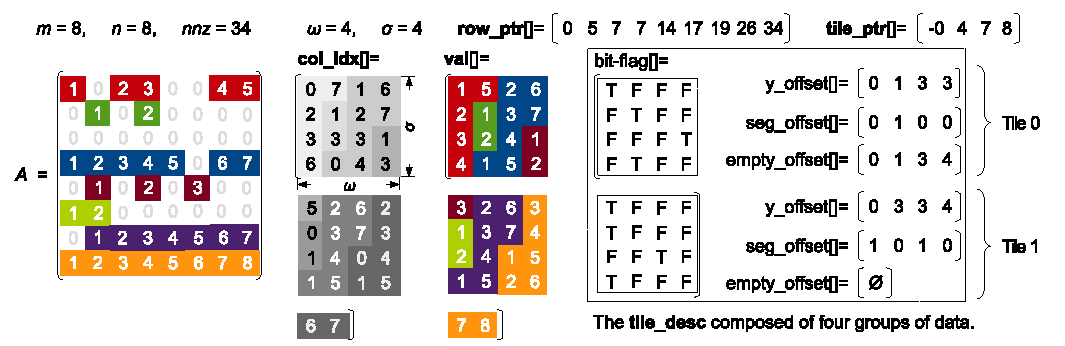
\includegraphics[scale=0.6]{A_csr5.pdf}
        \caption{Matrix A stored in CSR5 format (Source: CSR5).}
    \end{figure}
\end{frame}


\begin{frame}
    \frametitle{CSR5 SpMV (tile edition)}

    \begin{itemize}
        \item On modern CPUs with AVX2, \(\sigma\) and \(\omega\) can be set to $16$ and $4$ respectively and the whole tile can be
              processed in 16 iterations using AVX SIMD instructions.
    \end{itemize}

    \begin{figure}[htp]
        \centering
        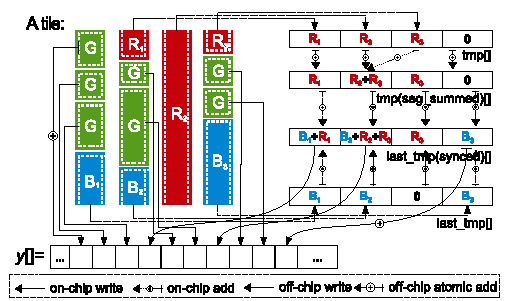
\includegraphics[scale=0.8]{A_secs.pdf}
        \caption{Sub-segments within a tile (Source: CSR5).}
    \end{figure}
\end{frame}


\begin{frame}
    \frametitle{CSR5 SpMV (shared memory system)}

    \begin{itemize}
        \item Each thread gets the same amount of tiles to process.
        \item Tiles are processed \textbf{sequentially} in the context of a thread (\csre{omp for static}).
        \item Not sensitive to the sparsity structure of the matrix (of course memory access patterns will still play a role).
    \end{itemize}

    \begin{figure}[htp]
        \centering
        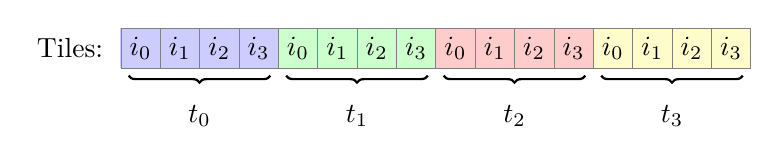
\begin{tikzpicture}
            % tiles

            \coordinate (tileArr) at (0, 0);

            % threads
            \filldraw[blue!20] ($ (tileArr) + (0, 0) $) rectangle ($ (tileArr) + (2, 0.5) $);
            \filldraw[green!20] ($ (tileArr) + (2, 0) $) rectangle ($ (tileArr) + (4, 0.5) $);
            \filldraw[red!20] ($ (tileArr) + (4, 0) $) rectangle ($ (tileArr) + (6, 0.5) $);
            \filldraw[yellow!20] ($ (tileArr) + (6, 0) $) rectangle ($ (tileArr) + (8, 0.5) $);

            \draw[step=0.5cm,gray,very thin] ($ (tileArr) + (0, 0) $) grid ($ (tileArr) + (8, 0.5)$);

            \foreach \x in {0,...,3}
                {
                    \coordinate (LLC\x) at ($(tileArr.west) + (\x * 2, 0)$);
                    \draw [
                        thick,
                        decoration={
                                brace,
                                mirror,
                                raise=0.1cm
                            },
                        decorate
                    ] ($(LLC\x) + (0.1, 0)$) -- ($ (LLC\x) + (2 - 0.1, 0) $)
                    node[pos=0.5,below=10pt,black]{$t_\x$};
                    \foreach \i in {0,...,3}
                    \node at ($(LLC\x) + (\i * 0.5 + 0.25, 0.25)$) {$i_\i$};
                }

            \node[anchor=east] at ($(tileArr) + (-0.1, 0.25)$) {Tiles:};
        \end{tikzpicture}
        \caption{Processing tiles using 4 threads}\label{csr5:thr_dist}
    \end{figure}
\end{frame}

\begin{frame}
    \frametitle{CSR5 synchronization}

    \begin{itemize}
        \item No synchronization necessary between tiles on the same thread (processed sequentially).
        \item A CSR5 tile may share only one output element in \csre{y} with a neighboring tile.
        \item Only the first output element in \csre{y} may be shared with the thread processing "previous" chunk of tiles.
        \item To avoid atomic operations, each thread has its own \csre{calibrator} where it stores this element until all threads are
              done. Then these contentious elements are added to \csre{y} sequentially.
    \end{itemize}
\end{frame}

% \begin{frame}
%     \frametitle{On-disk storage format}

%     \begin{overprint}
%         \begin{itemize}
%             \uncover<+->{ \item Recomputing CSR5 metadata every-time a matrix is loaded is expensive. }
%                   \uncover<+->{ \item CSR5 uses bit flags etc.\ so usual textual formats such as MMEF aren't suitable. }
%                   \uncover<+->{ \item Textual formats are also inherently slow to load because the values must be parsed by \csre{scanf} or a similar routine. }
%                   \uncover<+->{ \item Furthermore, the format should support loading the matrix only partially and support MPI-IO\@. }
%         \end{itemize}
%     \end{overprint}
% \end{frame}


% \begin{frame}
%     \frametitle{HDF5}
%     \begin{figure}
%         \centering
%         
\includegraphics[scale=0.1]{static/hdf.jpg}
%     \end{figure}
%     \begin{itemize}
%         \item Data model, library, and file format for storing and managing data.
%         \item Supports an unlimited variety of data types and is designed for flexible and
%               efficient I/O for high volume and complex data.
%         \item Supports loading datasets partially via hyperslabs.
%         \item Supports MPI-IO natively.
%     \end{itemize}
% \end{frame}

% \begin{frame}
%     \frametitle{HDF5 performance}
%     \begin{figure}
%         \centering
%         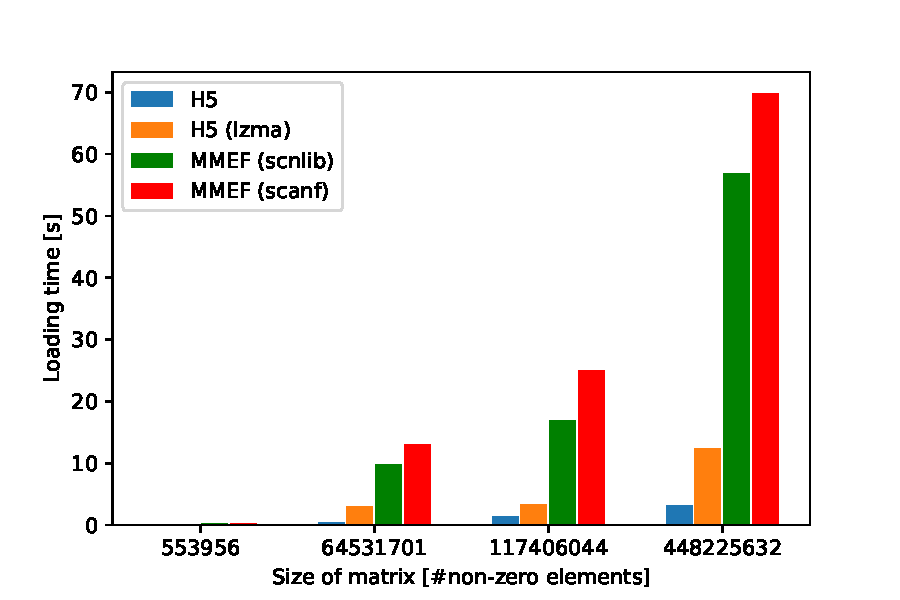
\includegraphics[scale=0.65]{static/mmef_vs_h5.pdf}
%     \end{figure}

% \end{frame}

\begin{frame}
    \frametitle{Distributed CSR5}
    \begin{itemize}
        \item Same principles apply. Just substitute threads with processes.
    \end{itemize}

    \begin{figure}[htp]
        \centering
        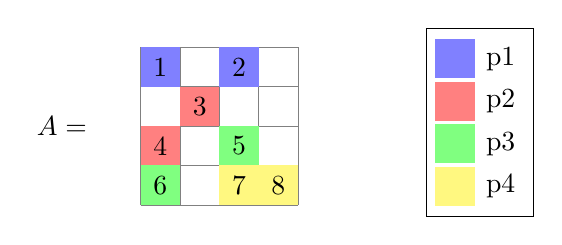
\begin{tikzpicture}[
                p1node/.style={rectangle, fill=blue!50, very thick, minimum size=5mm},
                p2node/.style={rectangle, fill=red!50, very thick, minimum size=5mm},
                p3node/.style={rectangle, fill=green!50, very thick, minimum size=5mm},
                p4node/.style={rectangle, fill=yellow!50, very thick, minimum size=5mm},
            ]

            \coordinate (ACoo) at (0, 0);

            \coordinate (yCoo) at (3 - 0.001, 1 - 0.001);

            \node at ($ (ACoo) + (-1, 1)$) {$A =$};

            % matrix
            \draw[step=0.5cm,gray,very thin] (ACoo) grid ($ (ACoo) + (2,2) $);

            % r0
            \node[p1node] at ($ (ACoo) + (0.25, 1.75) $) {1};
            \node[p1node] at ($ (ACoo) + (1.25, 1.75) $) {2};

            %r1
            \node[p2node] at ($ (ACoo) + (0.75, 1.25) $) {3};

            %r2
            \node[p2node] at ($ (ACoo) + (0.25, 0.75) $) {4};
            \node[p3node] at ($ (ACoo) + (1.25, 0.75) $) {5};

            %r3
            \node[p3node] at ($ (ACoo) + (0.25, 0.25) $) {6};
            \node[p4node] at ($ (ACoo) + (1.25, 0.25) $) {7};
            \node[p4node] at ($ (ACoo) + (1.75, 0.25) $) {8};


            \matrix [draw,below left] at (5, 2.25) {
                \node [p1node,label=right:p1] {}; \\
                \node [p2node,label=right:p2] {}; \\
                \node [p3node,label=right:p3] {}; \\
                \node [p4node,label=right:p4] {}; \\
            };
        \end{tikzpicture}
        \caption{Distribution of $A$ across 4 processes}
    \end{figure}

\end{frame}


\begin{frame}
    \frametitle{Distributed CSR5}
    \begin{itemize}
        \item Same case as if each process was multiplying a sub-matrix.
        \item Parallelization inside processes as in shared memory scenario.
    \end{itemize}

    \begin{figure}[htp]
        \centering
        \begin{tikzpicture}[
                p1node/.style={rectangle, fill=blue!50, very thick, minimum size=5mm},
                p2node/.style={rectangle, fill=red!50, very thick, minimum size=5mm},
                p3node/.style={rectangle, fill=green!50, very thick, minimum size=5mm},
                p4node/.style={rectangle, fill=yellow!50, very thick, minimum size=5mm},
            ]

            \coordinate (yCoo) at (3 - 0.001, 1 - 0.001);

            % r0
            \coordinate (p1) at (0, 0);
            \node[left=of p1, anchor=south] {$A_{p1}$};
            \draw[step=0.5cm,gray,very thin] (ACoo) grid ($ (p1) + (2,0.5) $);
            \node[p1node] at ($ (p1) + (0.25, 0.25) $) {1};
            \node[p1node] at ($ (p1) + (1.25, 0.25) $) {2};

            %r1
            \coordinate (p2) at (0, -1.5);
            \node[left=of p2, anchor=south] {$A_{p2}$};
            \draw[step=0.5cm,gray,very thin] (p2) grid ($ (p2) + (2.01, 1) $);
            \node[p2node] at ($ (p2) + (0.75, 0.75) $) {3};
            \node[p2node] at ($ (p2) + (0.25, 0.25) $) {4};

            %r2

            \coordinate (p3) at (5 - 0.01, -0.5);
            \node[left=of p3, anchor=south] {$A_{p3}$};
            \draw[step=0.5cm,gray,very thin] (p3) grid ($ (p3) + (2.01, 1) $);
            \node[p3node] at ($ (p3) + (1.25, 0.75) $) {5};
            \node[p3node] at ($ (p3) + (0.25, 0.25) $) {6};

            %r3
            \coordinate (p4) at (5 - 0.01, -1.5);
            \node[left=of p4, anchor=south] {$A_{p4}$};
            \draw[step=0.5cm,gray,very thin] (p4) grid ++(2.01, 0.5);
            \node[p4node] at ($ (p4) + (1.25, 0.25) $) {7};
            \node[p4node] at ($ (p4) + (1.75, 0.25) $) {8};
        \end{tikzpicture}
        \caption{Distribution of $A$ across 4 processes}
    \end{figure}

\end{frame}

\begin{frame}
    \frametitle{D-CSR5 synchronization}
    \begin{overprint}


        \begin{itemize}
            \item The sub-matrices still have overlapping elements.
                  \uncover<2-> {\item Simple solution, first process writing an element of $y$ "owns" it.}
        \end{itemize}

        \begin{figure}[htp]
            \centering
            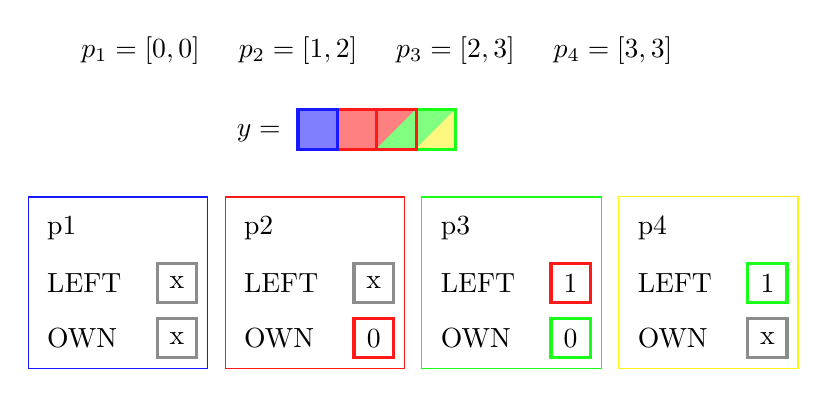
\begin{tikzpicture}[
                    p1node/.style={rectangle, fill=blue!50, very thick, minimum size=5mm},
                    p2node/.style={rectangle, fill=red!50, very thick, minimum size=5mm},
                    p3node/.style={rectangle, fill=green!50, very thick, minimum size=5mm},
                    p4node/.style={rectangle, fill=yellow!50, very thick, minimum size=5mm},
                    p1own/.style={rectangle, draw=blue!90, very thick, minimum size=5mm},
                    p2own/.style={rectangle, draw=red!90, very thick, minimum size=5mm},
                    p3own/.style={rectangle, draw=green!90, very thick, minimum size=5mm},
                    p4own/.style={rectangle, draw=yellow!90, very thick, minimum size=5mm},
                    node distance=7mm,
                    commst/.style={rectangle, very thick, minimum size=5mm, anchor=west},
                    tag/.style={minimum size=5mm, anchor=west},
                    commstnull/.style={rectangle, very thick, minimum size=5mm, draw=gray!90, anchor=west},
                ]

                \node at (1, 0.75) {$p_1 = [0, 0]$};
                \node at (3, 0.75) {$p_2 = [1, 2]$};
                \node at (5, 0.75) {$p_3 = [2, 3]$};
                \node at (7, 0.75) {$p_4 = [3, 3]$};

                \coordinate (yCoo) at (3, -0.5);
                \uncover<+->{
                    \node at ($ (yCoo) + (-0.5, 0.2) $) {$y = $};


                    % p1 output
                    \filldraw[blue!50] (yCoo) rectangle ($ (yCoo) + (0.5, 0.5)$);

                    % p2 output
                    \filldraw[red!50] ($(yCoo) + (0.5, 0) $) -- ($(yCoo) + (1, 0) $) -- ($ (yCoo) + (1.5, 0.5)$) -- ($ (yCoo) + (0.5, 0.5)$) -- cycle;

                    % p3 output
                    \filldraw[green!50] ($(yCoo) + (1, 0) $) -- ($(yCoo) + (1.5, 0) $) -- ($ (yCoo) + (2, 0.5)$) -- ($ (yCoo) + (1.5, 0.5)$) -- cycle;

                    % p4 output
                    \filldraw[yellow!50] ($(yCoo) + (1.5, 0) $) -- ($(yCoo) + (2, 0) $) -- ($ (yCoo) + (2, 0.5)$)-- cycle;

                    \draw[step=0.5cm,gray,very thin] (yCoo) grid ($ (yCoo) + (2 + 0.001, 0.5 + 0.001)$);
                }

                \uncover<+->{
                    \node[p3own] at ($(yCoo) + (1.75, 0.25)$) {};
                    \node[p2own] at ($(yCoo) + (1.25, 0.25)$) {};
                    \node[p2own] at ($(yCoo) + (0.75, 0.25)$) {};
                    \node[p1own] at ($(yCoo) + (0.25, 0.25)$) {};
                }

                \uncover<+->{
                    \node (p1) at (0, -1.5) {p1};

                    \node (p1lt) [below=of p1.west, tag] {LEFT};
                    \node (p1l) [right=1.5cm of p1lt.west, commstnull] {x};

                    \node (p1ot) [below=of p1lt.west, tag] {OWN};
                    \node (p1o) [below=of p1l.west, commstnull] {x};

                    \node [draw=blue!90, fit={(p1) (p1lt) (p1l) (p1o)}] {};

                    \node (p2) at (2.5, -1.5) {p2};

                    \node (p2lt) [below=of p2.west, tag] {LEFT};
                    \node (p2l) [right=1.5cm of p2lt.west, commstnull] {x};

                    \node (p2ot) [below=of p2lt.west, tag] {OWN};
                    \node (p2o) [below=of p2l.west, commst, style={draw=red!90}] {0};

                    \node [draw=red!90, fit={(p2) (p2lt) (p2l) (p2o)}] {};

                    \node (p3) at (5, -1.5) {p3};

                    \node (p3lt) [below=of p3.west, tag] {LEFT};
                    \node (p3l) [right=1.5cm of p3lt.west, commst, style={draw=red!90}] {1};

                    \node (p3ot) [below=of p3lt.west, tag] {OWN};
                    \node (p3o) [below=of p3l.west, commst, style={draw=green!90}] {0};

                    \node [draw=green!90, fit={(p3) (p3lt) (p3l) (p3o)}] {};

                    \node (p4) at (7.5, -1.5) {p4};

                    \node (p4lt) [below=of p4.west, tag] {LEFT};
                    \node (p4l) [right=1.5cm of p4lt.west, commst, style={draw=green!90}] {1};

                    \node (p4ot) [below=of p4lt.west, tag] {OWN};
                    \node (p4o) [below=of p4l.west, commstnull] {x};

                    \node [draw=yellow!90, fit={(p4) (p4lt) (p4l) (p4o)}] {};
                }
            \end{tikzpicture}
        \end{figure}
    \end{overprint}
\end{frame}

\begin{frame}
    \frametitle{D-CSR5 synchronization}

    \begin{figure}[htp]
        \centering
        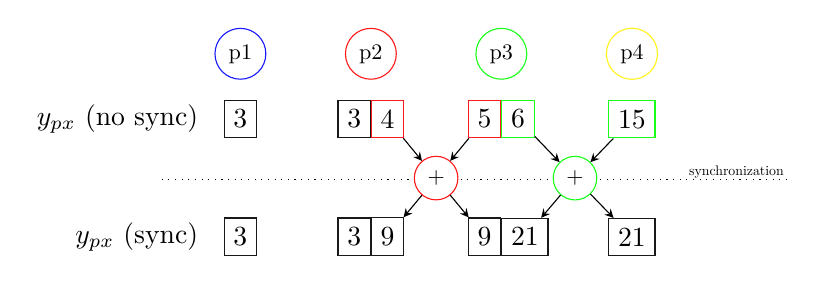
\begin{tikzpicture}[proc/.style={circle, minimum width=5mm, scale=0.8}]
            \node (p1) [proc, style={draw=blue!90}] {p1};
            \node (p2) [right=of p1, proc, style={draw=red!90}] {p2};
            \node (p3) [right=of p2, proc, style={draw=green!90}] {p3};
            \node (p4) [right=of p3, proc, style={draw=yellow!90}] {p4};

            \node (p11) [below=0.5cm of p1, rectangle, draw=black!90, anchor=center] {3};

            \node (p21) [below=0.5cm of p2, rectangle, draw=black!90, anchor=east] {3};
            \node (p22) [right=0cm of p21.east, rectangle, draw=red!90] {4};

            \node (p31) [below=0.5cm of p3, rectangle, draw=red!90,anchor=east] {5};
            \node (p32) [right=0cm of p31.east, rectangle, draw=green!90] {6};

            \node (p41) [below=0.5cm of p4, rectangle, draw=green!90, anchor=center] {15};

            \draw [dotted] (-1, -1.6) -- (7, -1.6);
            \node (st) [scale=0.5] at (6.3, -1.5) {synchronization};

            \node [left=0.2cm of p11, anchor=east] {$y_{px}$ (no sync)};

            \node (r23) [circle, fill=white!100, draw=red!90, minimum width=5mm, scale=0.8, anchor=center] at ($(p22)!0.5!(p31) + (0, -0.75)$) {$+$};
            \node (r34) [circle, fill=white!100, draw=green!90, minimum width=5mm, scale=0.8, anchor=center] at ($(p32)!0.5!(p41) + (0, -0.75)$) {$+$};

            \draw [-stealth] (p22) -- (r23);
            \draw [-stealth] (p31) -- (r23);

            \draw [-stealth] (p32) -- (r34);
            \draw [-stealth] (p41) -- (r34);

            \node (sp11) [below=1.25cm of p11, rectangle, draw=black!90, anchor=center] {3};

            \node (sp21) [below=1.25cm of p21, rectangle, draw=black!90, anchor=center] {3};
            \node (sp22) [below=1.25cm of p22, rectangle, draw=black!90, anchor=center] {9};

            \node (sp31) [below=1.25cm of p31, rectangle, draw=black!90, anchor=center] {9};
            \node (sp32) [right=0cm of sp31, rectangle, draw=black!90, anchor=west] {21};

            \node (sp41) [below=1.25cm of p41, rectangle, draw=black!90, anchor=center] {21};

            \node [left=0.2cm of sp11, anchor=east] {$y_{px}$ (sync)};


            \draw [-stealth] (r23) -- (sp22);
            \draw [-stealth] (r23) -- (sp31);

            \draw [-stealth] (r34) -- (sp32);
            \draw [-stealth] (r34) -- (sp41);
        \end{tikzpicture}
        \caption{Synchronization of result of \(Ax = y\) assuming \(x=1\)}
    \end{figure}
\end{frame}

\begin{frame}
    \frametitle{D-CSR5 result distribution}

    \begin{itemize}
        \item Uses \csre{MPI_Allgatherv}.
        \item Reuses \textbf{output ranges} which were needed for synchronization to compute \csre{recvcounts} and \csre{displs}.
        \item Only "owners" output contentious elements.
    \end{itemize}
    \begin{figure}[htp]
        \centering
        \begin{tikzpicture}[proc/.style={circle, minimum width=5mm, scale=0.8}]
            \node (p1) [proc, style={draw=blue!90}] {p1};
            \node (p2) [right=of p1, proc, style={draw=red!90}] {p2};
            \node (p3) [right=of p2, proc, style={draw=green!90}] {p3};
            \node (p4) [right=of p3, proc, style={draw=yellow!90}] {p4};

            \node (p11) [below=0.5cm of p1, rectangle, draw=black!90, anchor=center] {3};

            \node (p21) [below=0.5cm of p2, rectangle, draw=black!90, anchor=east] {3};
            \node (p22) [right=0cm of p21.east, rectangle, draw=black!90] {9};

            \node (p31) [below=0.5cm of p3, rectangle, draw=gray!90,anchor=east] {9};
            \node (p32) [right=0cm of p31.east, rectangle, draw=black!90] {21};

            \node (p41) [below=0.5cm of p4, rectangle, draw=gray!90, anchor=center] {21};

            \draw [dotted] (-1, -1.6) -- (7, -1.6);
            \node (st) [scale=0.5] at (6.3, -1.5) {\csre{MPI_Allgatherv}};

            \node [left=0.2cm of p11, anchor=east] {$y_{px}$ (sync)};


            \coordinate (res) at ($(p2)!0.5!(p3) + (0, -2.5)$);

            \node (sp1) [rectangle, draw=blue!90, anchor=center] at ($(res) + (-0.75, 0.25) $) {3};
            \draw [-stealth] (p11) -- (sp1);

            \node (sp2) [right=0cm of sp1.east, rectangle, draw=red!90, anchor=west] {3};
            \draw [-stealth] (p21) -- (sp2);

            \node (sp3) [right=0cm of sp2.east, rectangle, draw=red!90, anchor=west] {9};
            \draw [-stealth] (p22) -- (sp3);

            \node (sp4) [right=0cm of sp3.east, rectangle, draw=green!90, anchor=west] {21};
            \draw [-stealth] (p32) -- (sp4);

            \node [left=0.2cm of sp11, anchor=east] {$y$ (sync)};
        \end{tikzpicture}
        \caption{Distribution of result of \(Ax = y\) assuming \(x=1\)}
    \end{figure}
\end{frame}

\begin{frame}
    \frametitle{Benchmarks - specification}

    \begin{itemize}
        \item D-CSR5 and PETSc based implementations.
        \item Portable, Extensible Toolkit for Scientific computation (PETSc) is a suite of
              data structures and routines for scalable solutions of scientific applications
              modeled by partial differential equations

    \end{itemize}

    \centering
    \begin{tabular}{|c|c|c|c|}
        \hline
        \textbf{name}      & \textbf{n}      & $n_{nz}$         & \textbf{CSR5 on-disk size} [GiB] \\
        \hline
        \hline
        \textbf{nlpkkt240} & \num{27993600}  & \num{774472352}  & 9.1                              \\
        \hline
        \textbf{GAP-web}   & \num{50636151}  & \num{1930292948} & 22.6                             \\
        \hline
        \textbf{GAP-kron}  & \num{134217726} & \num{4223264644} & 49.6                             \\
        \hline
    \end{tabular}
    \begin{itemize}
        \item Each implementation will load matrix $A$ and perform 100 iterations of \textbf{conjugate
                  gradient method}, trying to find $x$ satisfying $Ax=1$.
        \item Every step of \textbf{conjugate gradient} iteration is kept track of.
    \end{itemize}
\end{frame}


\begin{frame}
    \frametitle{Benchmarks - why bechmark on CG?}

    \begin{itemize}
        \item Iterative nature makes obtaining statistically relevant sample simple.
        \item Real world use-case of SpMV\@.
        \item SpMV is by far the most computationally intensive step.
    \end{itemize}

    \begin{figure}[htp]
        \centering
        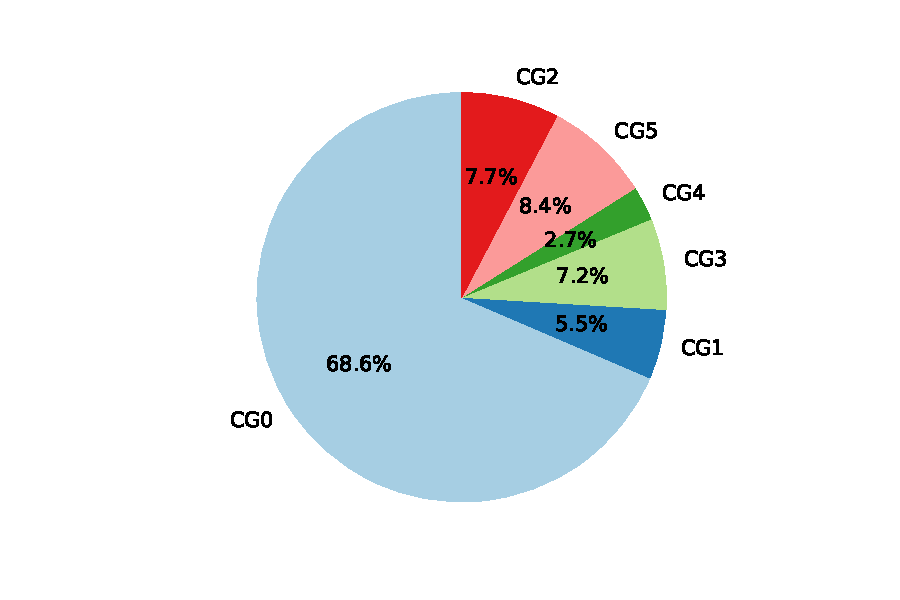
\includegraphics[scale=0.45]{static/cg_sp_nlpkkt240_16.pdf}
        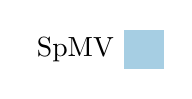
\begin{tikzpicture}
            \node (p1) [style={fill=SpMVCGS}, minimum size=5mm, label=west:SpMV] at (0, 0) {};
        \end{tikzpicture}
        \caption{Average percentage of time spent in steps of single iteration. \textbf{nlpkkt240} with \textbf{16} threads.}
    \end{figure}
\end{frame}


\begin{frame}
    \frametitle{Benchmarks - hardware/compiler}

    \begin{overprint}
        \begin{itemize}
            \uncover<+-> {
            \item Ran on RCI cluster (AMD nodes).
            \item \textbf{CPU}: \texttt{2 x (AMD EPYC 7543 32C/64T @3.1GHz) } \\
                  \textbf{Network}: \texttt{200GbE InfiniBand EDR} \\
                  \textbf{RAM}: \texttt{1TB} \\
                  \textbf{Storage}: \texttt{8TB NVMe} \\
                  \textbf{Compiler}: \texttt{GCC 10.3} \\
                  \textbf{Optimization level}: \texttt{-O3} \\
                  \textbf{March}: \texttt{native(znver2)} \\
                  }
                  \uncover<+->{
            \item A layout in this text will mean a triplet of \textbf{node count} $N$,
                  \textbf{number of processes per node} $P$
                  and \textbf{number of CPUs per process} $C$ (usually abbreviated to \csre{N-P-C}).
                  }
        \end{itemize}
    \end{overprint}

\end{frame}


% \begin{frame}
%     \frametitle{Benchmarks - CSR5}
%     \begin{figure}[htp]
%         \centering
%         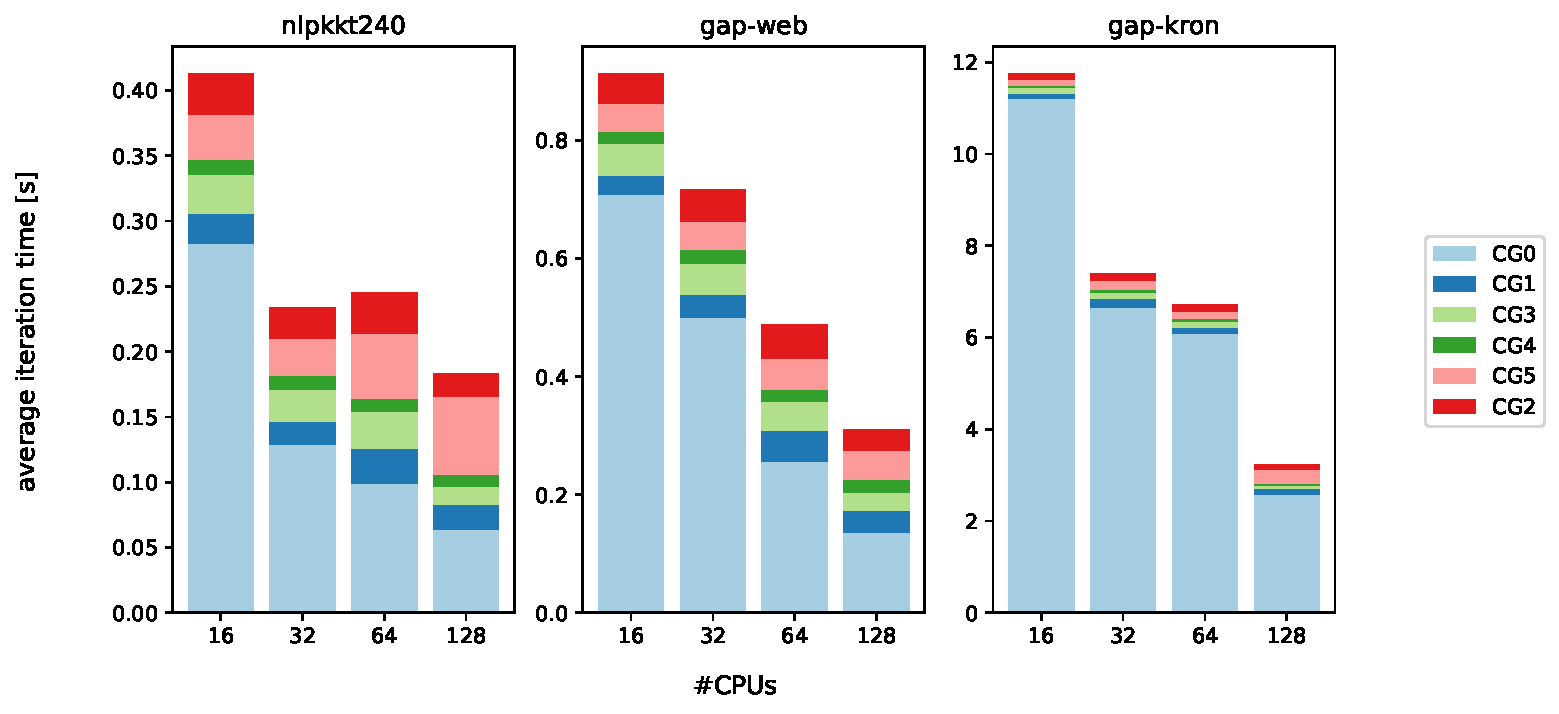
\includegraphics[scale=0.4]{static/single_process.pdf}
%     \end{figure}
% \end{frame}



\begin{frame}
    \frametitle{Benchmarks - CSR5 vs D-CSR5}
    \begin{figure}[htp]
        \centering
        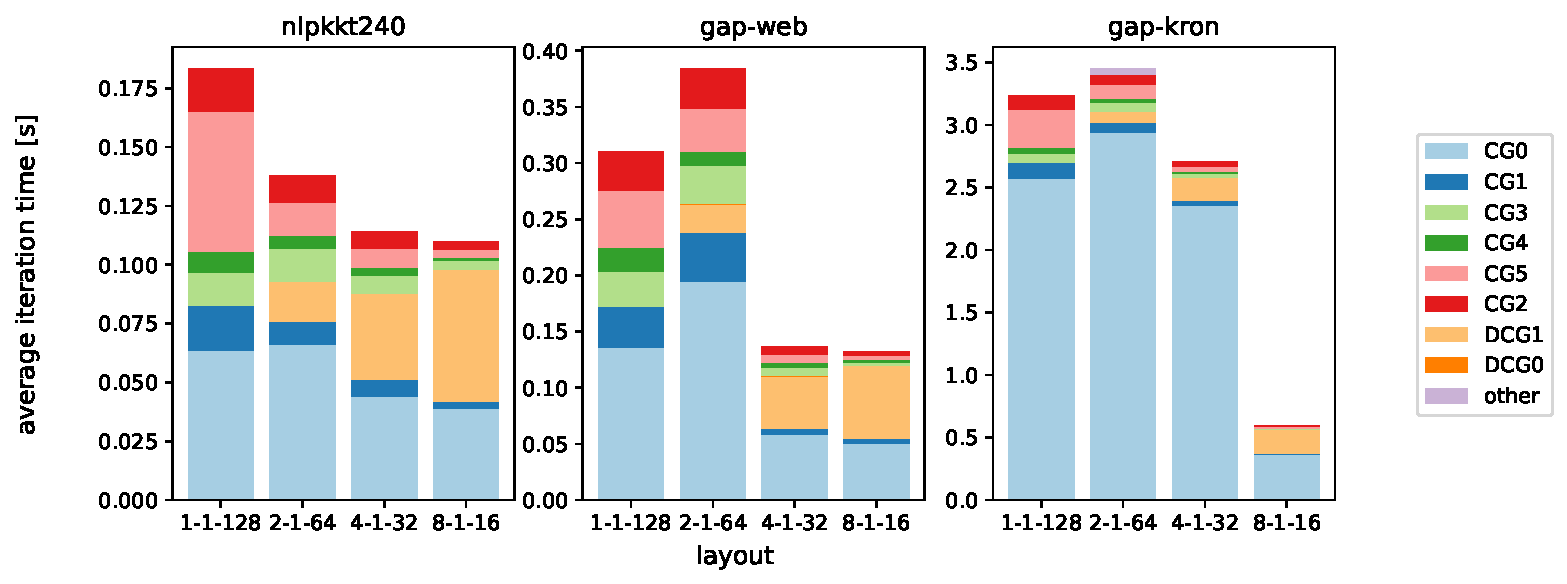
\includegraphics[scale=0.45]{static/mpi.pdf}
    \end{figure}
    \centering
    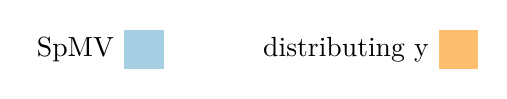
\begin{tikzpicture}
        \node (p1) [style={fill=SpMVCGS}, minimum size=5mm, label=west:SpMV] at (0, 0) {};
        \node (p2) [style={fill=SpMVDISTS}, minimum size=5mm, label=west:{distributing y}] at(4, 0) {};
    \end{tikzpicture}
\end{frame}

\begin{frame}
    \frametitle{Benchmarks - PETSc}
    \begin{itemize}
        \item Because of how PETSc is designed, when creating a sub-vector from $y$, it \textbf{may} be copied, thus
              skewing the results as synchronization is now the most computationally heavy part of iteration.
        \item The synchronization time (DCG1) is discarded for the following comparison.
    \end{itemize}
    \begin{figure}[htp]
        \centering
        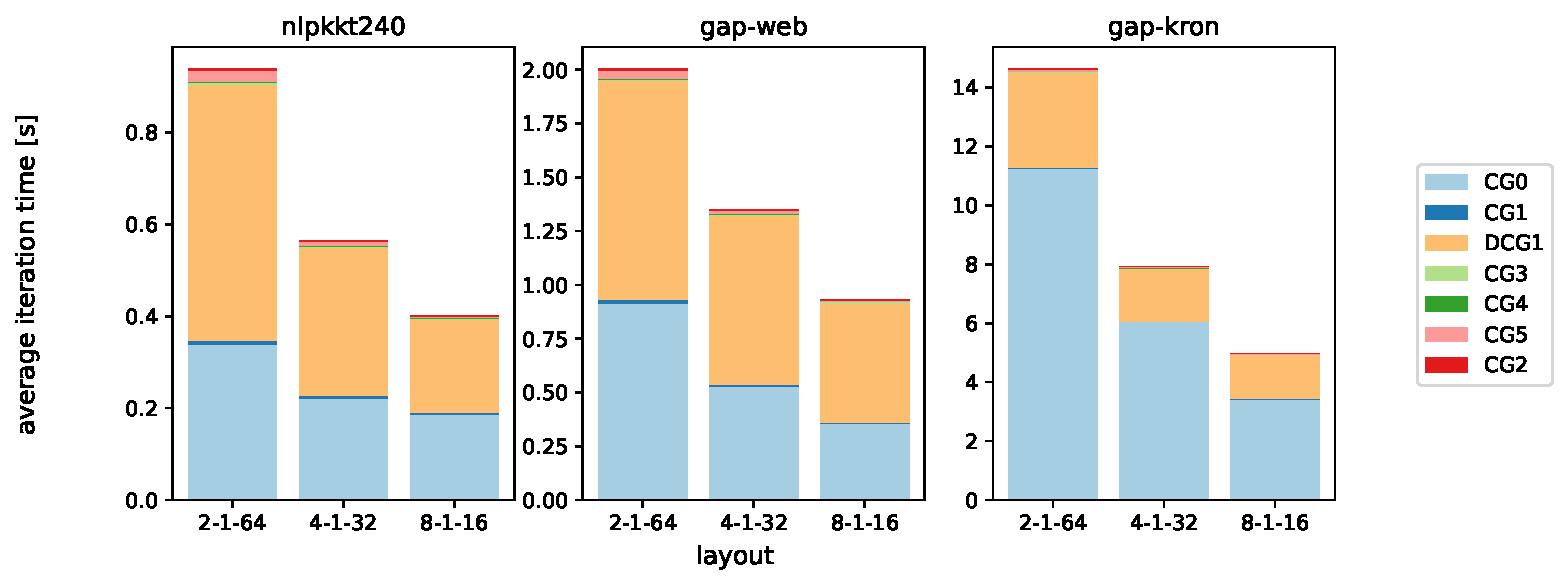
\includegraphics[scale=0.45]{static/petsc_mpi.pdf}
    \end{figure}
\end{frame}

\begin{frame}
    \frametitle{Benchmarks - PETSc vs D-CSR5}
    \begin{figure}[htp]
        \centering
        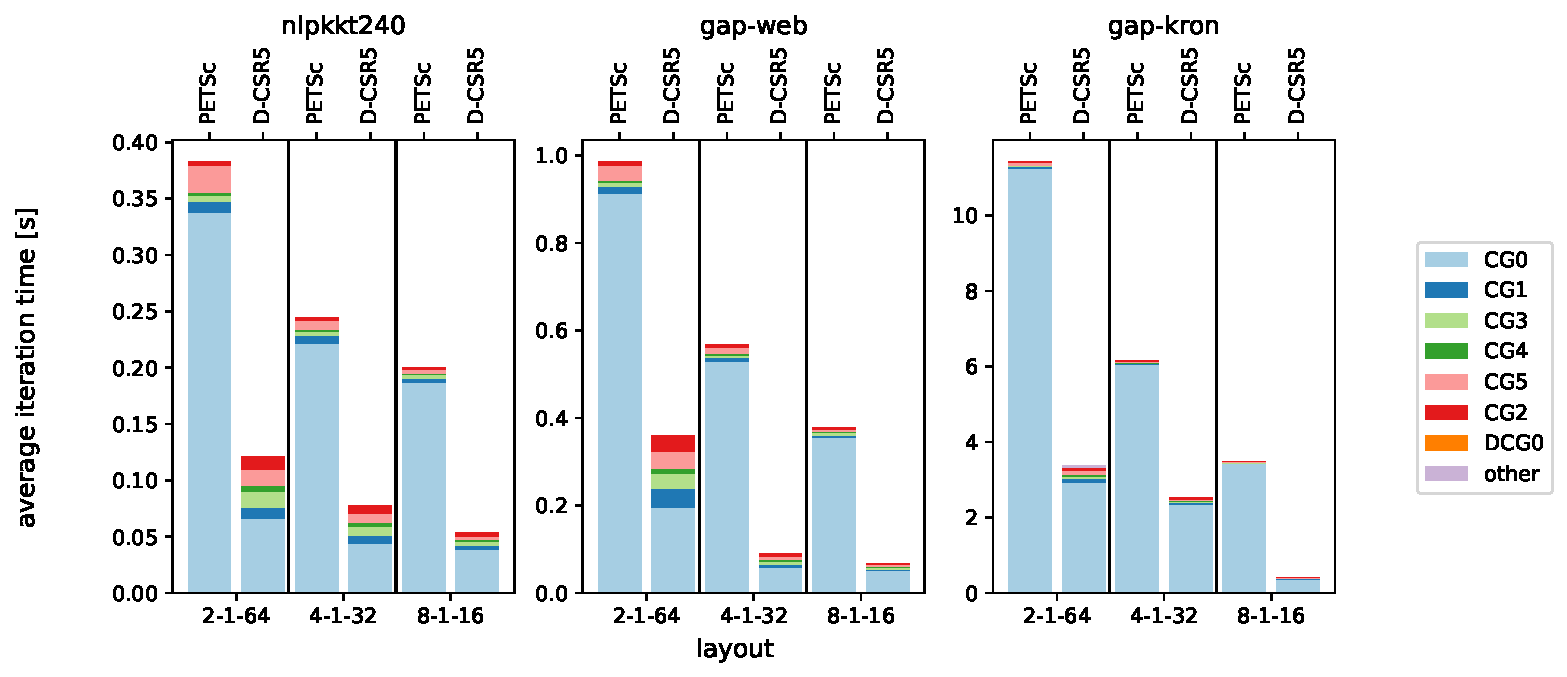
\includegraphics[scale=0.45]{static/petsc_vs_dim.pdf}
    \end{figure}
    \begin{itemize}
        \item D-CSR5 implementation performs better on all the benchmarked configurations.
        \item The speedup ranges from 2.57x up to 9.46x.
    \end{itemize}
\end{frame}

\begin{frame}
    \frametitle{Conclusion}
    \begin{itemize}
        \item CSR5 scales up to distributed systems very well.
        \item Only small changes in regards to synchronization needed.
        \item Distributed approach leads to non-negligible speedups for large matrices.
        \item More research on heterogeneous implementations (CPU + GPU)?
    \end{itemize}
\end{frame}

\begin{frame}
    \frametitle{Opponents remarks}
    \begin{overprint}
        \begin{itemize}
            \item Do jak velké míry jste musel přepsat stávající implementaci formátu CSR5 a doprovodnou implementaci pro násobení řídké matice vektorem, abyste získal distribuovanou implementaci popisovanou v ZP?
            \item Stačilo provést drobné úpravy v úzce vymezených částech stávající implementace či bylo potřeba výrazným způsobem stávající implementaci přepisovat?
                  \only<1>{\item Nebo jste celou stávající implementaci CSR5 přepsal od začátku?}
                  \only<2>{\item \textcolor{green}{Nebo jste celou stávající implementaci CSR5 přepsal od začátku?}}
        \end{itemize}
    \end{overprint}
\end{frame}

\begin{frame}
    \frametitle{Opponents remarks}

    \begin{outline}
        \1 CSR5 storage format and its accompanying SpMV algorithm needed only minimal modifications to make it distributed.
        Namely the addition of ownership rules and synchronization communicators described in previous slides.
        \1 However, the C++ implementation in this thesis is bespoke for several reasons:
        \2 There were some alignment issues in the original implementation.
        \2 Since the code uses SIMD intrinsics and tries to be as branchless as possible, it is quite hard to debug and fix without a good
        understanding of these techniques.
        \2 It is from 2015, C++20 introduced a lot of features immediately relevant for this problem space.
    \end{outline}
\end{frame}

\begin{frame}
    \frametitle{dim}
    \begin{itemize}
        \item \csre{dim} is a library which is a byproduct of this thesis.
        \item Contains routines for working with COO, CSR and CSR5 formats (SpMV as well as I/O).
        \item `Modern' C++ HDF5 API (official HDF5 C++ bindings don't support MPI-IO).
        \item \csre{dim_cli} command line interface which can convert between formats, generate structural maps etc.
    \end{itemize}
\end{frame}

\begin{frame}
    \centering \Huge
    \emph{Thank you for your attention!} \\
    \Large
    Any questions?
\end{frame}


\end{document}